%
% Simple asymmetric two-column CV
% Author: Sofia JIJON
%

\documentclass[a4paper,10pt]{article}
\usepackage[vmargin=1.2cm, hmargin=1.5cm]{geometry}
% !TEX root = Simple-CV.tex
%-------------------------------------------------------------------------------------------------------
% Packages
%-------------------------------------------------------------------------------------------------------
% \usepackage[latin1]{inputenc}
\usepackage[T1]{fontenc}
\usepackage[english]{babel}
\usepackage{fontawesome}
\usepackage{datetime}
\usepackage[usenames,dvipsnames]{xcolor}
\usepackage[colorlinks=true, urlcolor=ColorTwo]{hyperref}
\usepackage{tikz}
\usepackage{hyperref}
\usepackage{setspace}
\usepackage{graphicx}
\usepackage{enumitem}
\usepackage{sectsty}
\usepackage{multicol}
\usepackage{adjustbox}
\usepackage{setspace}
%-------------------------------------------------------------------------------------------------------
% Layout
%-------------------------------------------------------------------------------------------------------
\pagenumbering{gobble}
\renewcommand{\baselinestretch}{1.5}
% \inputencoding{utf8}
\setmainfont{Liberation Serif}
% \setmainfont{DejaVu Sans}

%
% Color theme
%
\definecolor{ColorOne}{RGB}{115,19,13} 	% Blue
\definecolor{ColorTwo}{RGB}{120,0,120} 	% Mauve
\definecolor{Cyan}{RGB}{0,255,255} 	% Mauve
\definecolor{mycyan}{RGB}{0,255,255} 	% Mauve
\definecolor{Purple}{RGB}{255,0,255} 	% Mauve
%\definecolor{ColorTwo}{RGB}{140,100,0} 	% Gold

\sectionfont{\color{ColorOne}}
\subsectionfont{\color{ColorOne}}

%
% Vertical line
%
\newcommand{\MyVerticalRule}{%
	\textcolor{ColorOne}{\rule{1pt}{\textheight}}
}

%
% Update
%
\newcommand{\LastUpdate}{%
\vfill
\centering \small
\textcolor{ColorOne}{Last updated: \monthname,~\the\year.}
}

%
% Skip
%
\newcommand{\MySkip}{
\vskip12pt
}

%
% Format hyperrefs
%
\newcommand{\myhref}[2]{%
\href{#1}{\textcolor{Purple}{#2}}
}
%
% Format skill bullets
%
\newcommand{\SkillBull}[1]{%
\textcolor{ColorTwo}{#1}
}

\newcommand{\mpwidth}{\linewidth-\fboxsep-\fboxsep}
\definecolor{maincol}{RGB}{ 45, 50, 90 }
\definecolor{lightcol}{RGB}{245,245,245}
\definecolor{Orange}{RGB}{250,76,67}

\newcommand{\cvskill}[2][0.85] {
    \newcommand{\height}{0.20}
    \hspace{-2.7mm}
	\begin{tikzpicture}
	    \draw[rounded corners=0.2mm][preaction={draw, line width=0.6mm, black}][clip] (0,0) rectangle (#1\mpwidth, \height);
	    \fill [lightcol] (0,0) rectangle (#1\mpwidth, \height);
	    \fill [Orange] (0,0) rectangle (#2*#1\mpwidth, \height);
		% \clip[postaction={fill=mycyan, draw=black, line width=0.5mm}] (0,0) rectangle +(#1\mpwidth,0.15);
	\end{tikzpicture}\\%
}


% \usepackage{titlesec}

%-------------------------------------------------------------------------------------------------------

\begin{document}
\thispagestyle{empty}

%-------------------------------------------------------------------------------------------------------
% Left column
%-------------------------------------------------------------------------------------------------------
\begin{adjustbox}{valign=t}
\begin{minipage}{0.3\textwidth} % Adapt width to your convenience
%----------------------------------------------------
% Please add a photo in 1x1 format
\begin{center}
\begin{tikzpicture}
	\clip (0,0) circle (2cm) node {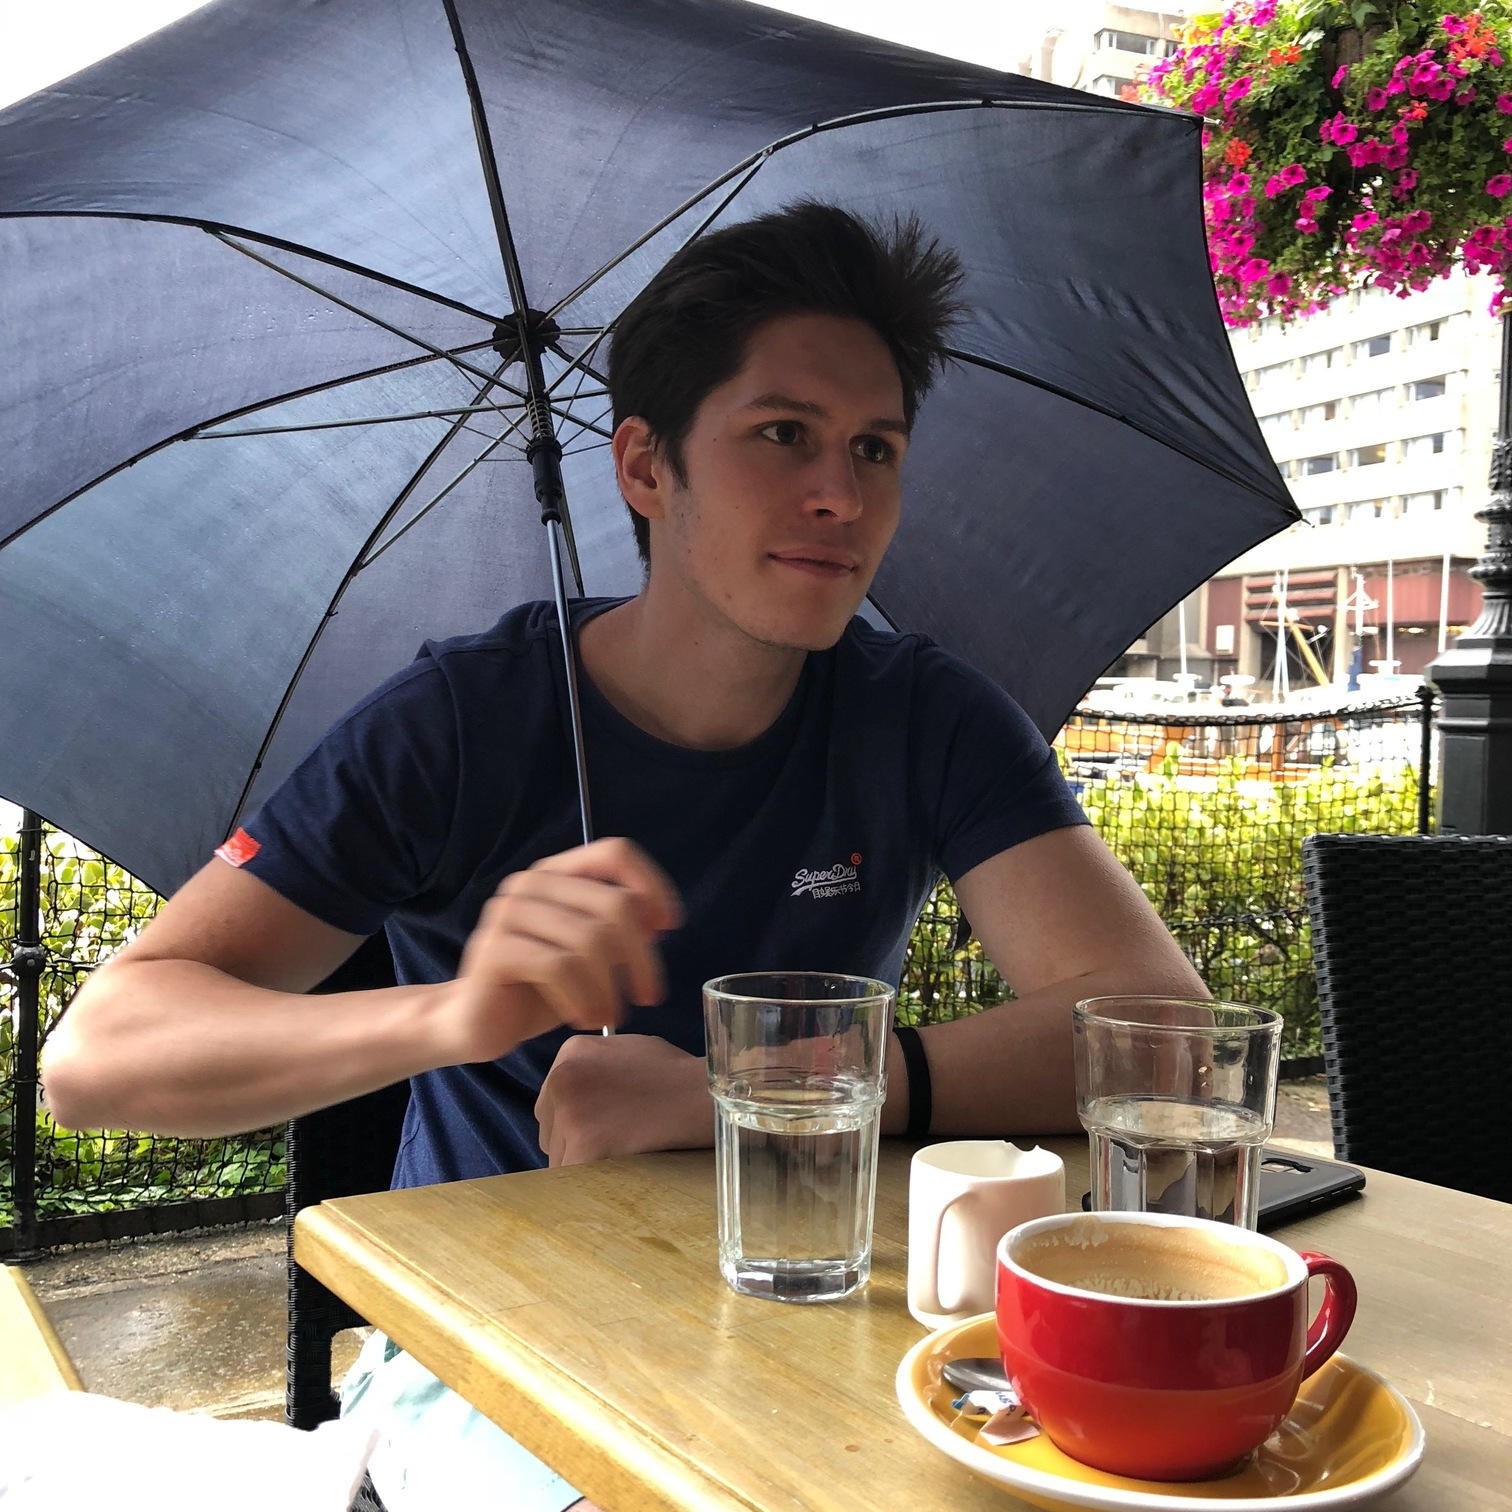
\includegraphics[width=4cm]{IMG_4442}};
\end{tikzpicture}

\MySkip 	% See MySetup.tex file

%----------------------------------------------------
\raggedright
{\LARGE \bfseries Pierre-Louis Braun}

\MySkip 	% See MySetup.tex file

\begin{spacing}{1.0}
Born on July 13th, 1998\\
Mulhouse -- France\\
Currently living in Delémont Switzerland\\
\end{spacing}
% J'aime mon petit coeur <3\\

\MySkip 	% See MySetup.tex file

\textcolor{ColorTwo}{\faEnvelopeO}
\myhref{mailto:plbraundev@gmail.com}{plbraundev@gmail.com} \\
\vspace{-1.5\baselineskip}

% \textcolor{ColorTwo}{\faChain}
% \myhref{https://alkeryn.com}{https://alkeryn.com}
\end{center}

\vfill

%----------------------------------------------------
\section*{Personal Interests}
\raggedright
\begin{spacing}{1.0}
\textcolor{ColorOne}{$\circ$} Computers\\
\textcolor{ColorOne}{$\circ$} Science\\
\textcolor{ColorOne}{$\circ$} Physics\\
\textcolor{ColorOne}{$\circ$} AI\\
\textcolor{ColorOne}{$\circ$} Hacking / Cybersecurity\\
\end{spacing}

\vfill
%----------------------------------------------------
\section*{Work Experience}
\begin{description}
		\begin{spacing}{1.0}
		\item [\normalfont \textcolor{ColorOne}{10/2022 - 07/2023.}] \textbf{Everdreamsoft}\\
			Working as a Full Stack developer for Everdreamsoft\\
			Geneva -- Switzerland
		\item [\normalfont \textcolor{ColorOne}{9/2021 - NOW.}] \textbf{Self Employed}\\
			Working at my own company\\
			Mulhouse -- France
		\item [\normalfont \textcolor{ColorOne}{07/2022 - 10/2022.}] \textbf{Sogeti}\\
			Working as a cybersecurity consultant for the PSA Finance bank
			as a service provider for Sogeti\\
			Meroux -- France
		\end{spacing}
\end{description}
\vspace{-2\baselineskip}
%----------------------------------------------------
\section*{Education}
\begin{description}
		\raggedright
	\item [\normalfont \textcolor{ColorOne}{2017 - 2020.}] \textbf{UHA 4.0}\\
		Computer Science University\\
		Mulhouse -- France
	\item \textbf{Lycée Blaise Pascal Colmar}\\
		Highschool\\
		Colmar -- France

	\item \mbox{\textbf{Collège Jaques Prévert}}\\
		Middle school \\
		France
\end{description}

\vfill
\end{minipage}
\end{adjustbox}
%
%
%-------------------------------------------------------------------------------------------------------
% Vertical rule
%-------------------------------------------------------------------------------------------------------
%
\hfill
\begin{adjustbox}{valign=t}
\begin{minipage}{0.05\textwidth} % Adapt width to your convenience
\MyVerticalRule  % See MySetup.tex file
\end{minipage}
\end{adjustbox}
\hfill
%
%-------------------------------------------------------------------------------------------------------
% Right column
%-------------------------------------------------------------------------------------------------------
\begin{adjustbox}{valign=t}
\begin{minipage}{0.6\textwidth} % Adapt width to your convienience
\section*{Current situation:}
\begin{description}
\raggedright
\item[\normalfont \textcolor{ColorOne}{August. 2023 -- Now.}] \textbf{Looking for a job}\\ \medskip

	\begin{spacing}{1.0}
		I'm working on my company and personal projects in the meanwhile.\\
		I'd love to do Rust for my next Job.
	\end{spacing}

\vspace{-0.9\baselineskip}
\end{description}

%----------------------------------------------------
\section*{Bio:}
\begin{spacing}{1.0}

\vspace{-0.6\baselineskip}

\hspace{5mm} I'm a computer hobbyist since the age of 9, I've been learning computer science,
programming languages and various technologies since.\\
I don't have many diplomas but i can show my skills.
\end{spacing}
\vspace{-0.8\baselineskip}
%----------------------------------------------------
\section*{Recommendations:}
\vspace{-0.2\baselineskip}
\begin{spacing}{0.8}
\begin{description}
	\item{\textbf{Ali Anwar:}}\\
		CTO at \textbf{Everdreamsoft}\\
		+41789052972
\end{description}

\vspace{-4.0\baselineskip}
\end{spacing}
%----------------------------------------------------
\section*{Skills:}
\begin{description}
\begin{spacing}{0.85}
\item{\textbf{Languages:}}

	\textbf{C} | C++20 | ASM x86 \& ARM | \textbf{Python} | \textbf{Rust} \\
		\textbf{Bash} | ZSH | Vim, Vimscript | Make | Cmake | Awk\\
    HTML5, css, Javascript | NodeJs | PHP | Go\\
    Ruby | Java | Kotlin | Dart\\
    Haskell | Lisp | Lua | Ada, Ada Sparks | Zig | Wasm\\
    Julia | R | Cobol | Fortran \\
    Markdown | \LaTeX | XML | YAML | JSON

\item{\textbf{Tools / Software:}}

    GNU coreutils, gdb, radare2, ghidra, ida pro, frida, sed, nmap\\
    metasploit framework, bettercap, netcat, netstat, ip, ss\\
    \{s,m,l\}trace, objdump, xxd, ld, ldd, wireshark, tshark, tcpdump {[..]}

\item{\textbf{Sysadmin skills:}}

    Linux, Unix | KVM | Qemu | Libvirt | Docker | LXC, LXD\\
    Nix | Kubernetes | ZFS | Btrfs\\
    Regex, globs \& wildcards\\
    Systemd | systemd-nspawn | machinectl

\item{\textbf{Technology:}}

    Git | UML | Graphviz | Ajax | Arduino | Jira | Confluence\\
    SQL: mysql, postgres | NoSQL: mongodb, redis, scylladb\\
    NewSQL: cockroachDB | Nginx

\item{\textbf{Libraries:}}

    SDL2 , SFML, OpenGL, Vulkan\\
    Ncurses, QT, GTK, Tk, XCB\\
    Opencl, Sycl, Hip, OpenACC/OpenMP, Cuda\\
    socket, libssh, libsodium, STD \& STL algorithm{[...]}

\item{\textbf{Misc:}}

    Cybersecurity, Reverse engineering, Binary exploitation\\
    Forensic analysis, Cryptanalysis, Data Oriented Programming\\
    AI, Machine learning and expert systems.\\
    Android JDK, Android NDK | Computer Architecture\\
    Arch Linux, Gentoo, LFS(linux from scratch), NixOS, Debian

\vspace{-2.2\baselineskip}
\end{spacing}
\end{description}

% \section*{Experience}
% \begin{description}
% \raggedright
% \item[\normalfont \textcolor{ColorOne}{Sep. 2017 -- Aug. 2018.}]
% 	\textbf{Your previous job}\\ \medskip

% 	Your previous employer\\

% 	Here you describe what you did before working where you are working now.

% \item[\normalfont \textcolor{ColorOne}{Sep. 2012 -- Aug. 2017.}]
% 	\textbf{Your first job}\\ \medskip

% 	Your employer\\

% 	This could be a nice short description of your first job.
% \end{description}

%----------------------------------------------------
\section*{Achievements}
\begin{spacing}{1.0}
    \raggedright
    One of the winners of the DGSE Richelieu hacking CTF \textbf{(2019)}
\end{spacing}
\vspace{-1.0mm}
%----------------------------------------------------
% \section*{Oral communications}
% \begin{description}
% 	\raggedright
% 	\item \underline{Name, Y.}, Second Author, N., Third Author, N. et al. \textbf{(2019)} The title of a talk you did. {\it Conference}, November 16, 2006, City, Country.
% \end{description}
%----------------------------------------------------
% \section*{Another section}
% \begin{description}
% 	\raggedright
% 	\item Something you want to include in your CV
% \end{description}

% \MySkip
%----------------------------------------------------
\setlength{\columnsep}{-2cm}
\begin{multicols}{2}

\section*{Languages}
\begin{tabular}{ll}
    French & \cvskill[0.3]{1}
    English & \cvskill[0.3]{0.95}
\end{tabular}

\vfill\null \columnbreak  % Break column for new section

\section*{Hobbies}

\begin{spacing}{0.9}
Cooking | Programming | Hacking | Painting\\
Listening to music | Hiking | Electronic\\
Learning | Reading | Sport | Skateboarding
\end{spacing}

\vfill\null  % Break column for new section

\end{multicols}
\vspace{-1\baselineskip}

% \begin{spacing}{0.8}
%     \begin{tabular}{ll}
% 	Rust & \cvskill {1.0}\\
% 	C & \cvskill {0.6}\\
% 	petit coeur & \cvskill {1}\\
%     \end{tabular}
% \end{spacing}
%----------------------------------------------------
\LastUpdate

\vfill
\begin{flushright}
    This resume was made using \LaTeX
\end{flushright}
%----------------------------------------------------
\end{minipage}
\end{adjustbox}
\newpage
\section*{Personal projects:}
\begin{spacing}{1}
	\subsection*{\textcolor{purple}{Virtablet app:}}
	Virtablet was an app that allowed you to use any android tablet with the required hardware like a cintiq graphic tablet (including video transfer and multitouch) on windows and Linux computers
	(mac and ipad support would be added later);\\

	To do so, a kotlin android app was made, it registered the events (position, pressure, tilt, orientation, multitouch) then sent them over the network using a custom protocol over tcp and udp.
	on the computer side i had to write a server to receive and inject the event, the server was initially written in C++ and the networking was done with tcp and udp sockets, i used \#ifdefs for linux and windows compatibility as i made my own networking library, however i later rewrote the whole thing in \textbf{Rust}.
	then once the packets were received and the events parsed from my custom format, i had to inject them; since windows doesn't have any syscalls for input injection, i had to develop a driver using
	\textbf{KMDF} so that i'd be able to create a "virtual graphic tablet" to which i'd send pen and multitouch events.\\

	on Linux on the other hand, i didn't need to write a driver and could just use \textbf{libinput}, basically allowing you to create virtual devices with ioctls where you define what kind of device it is and its varius parameters, and then sending the events to that device.
	\\
	\\
	Network discovery was made using udp broadcast.\\

	Only the video transfer part was left to do, but unfortunately someone made the same software and released it only a few weeks before my planned release date, i contacted the developper behind it
	and like me he was an independant, however he started working on the project two years earlier.

	\noindent as the app lost most commercial viability, i never finished the project and moved on to something else.

	\begin{figure}[h!]
		\noindent\makebox[\textwidth]{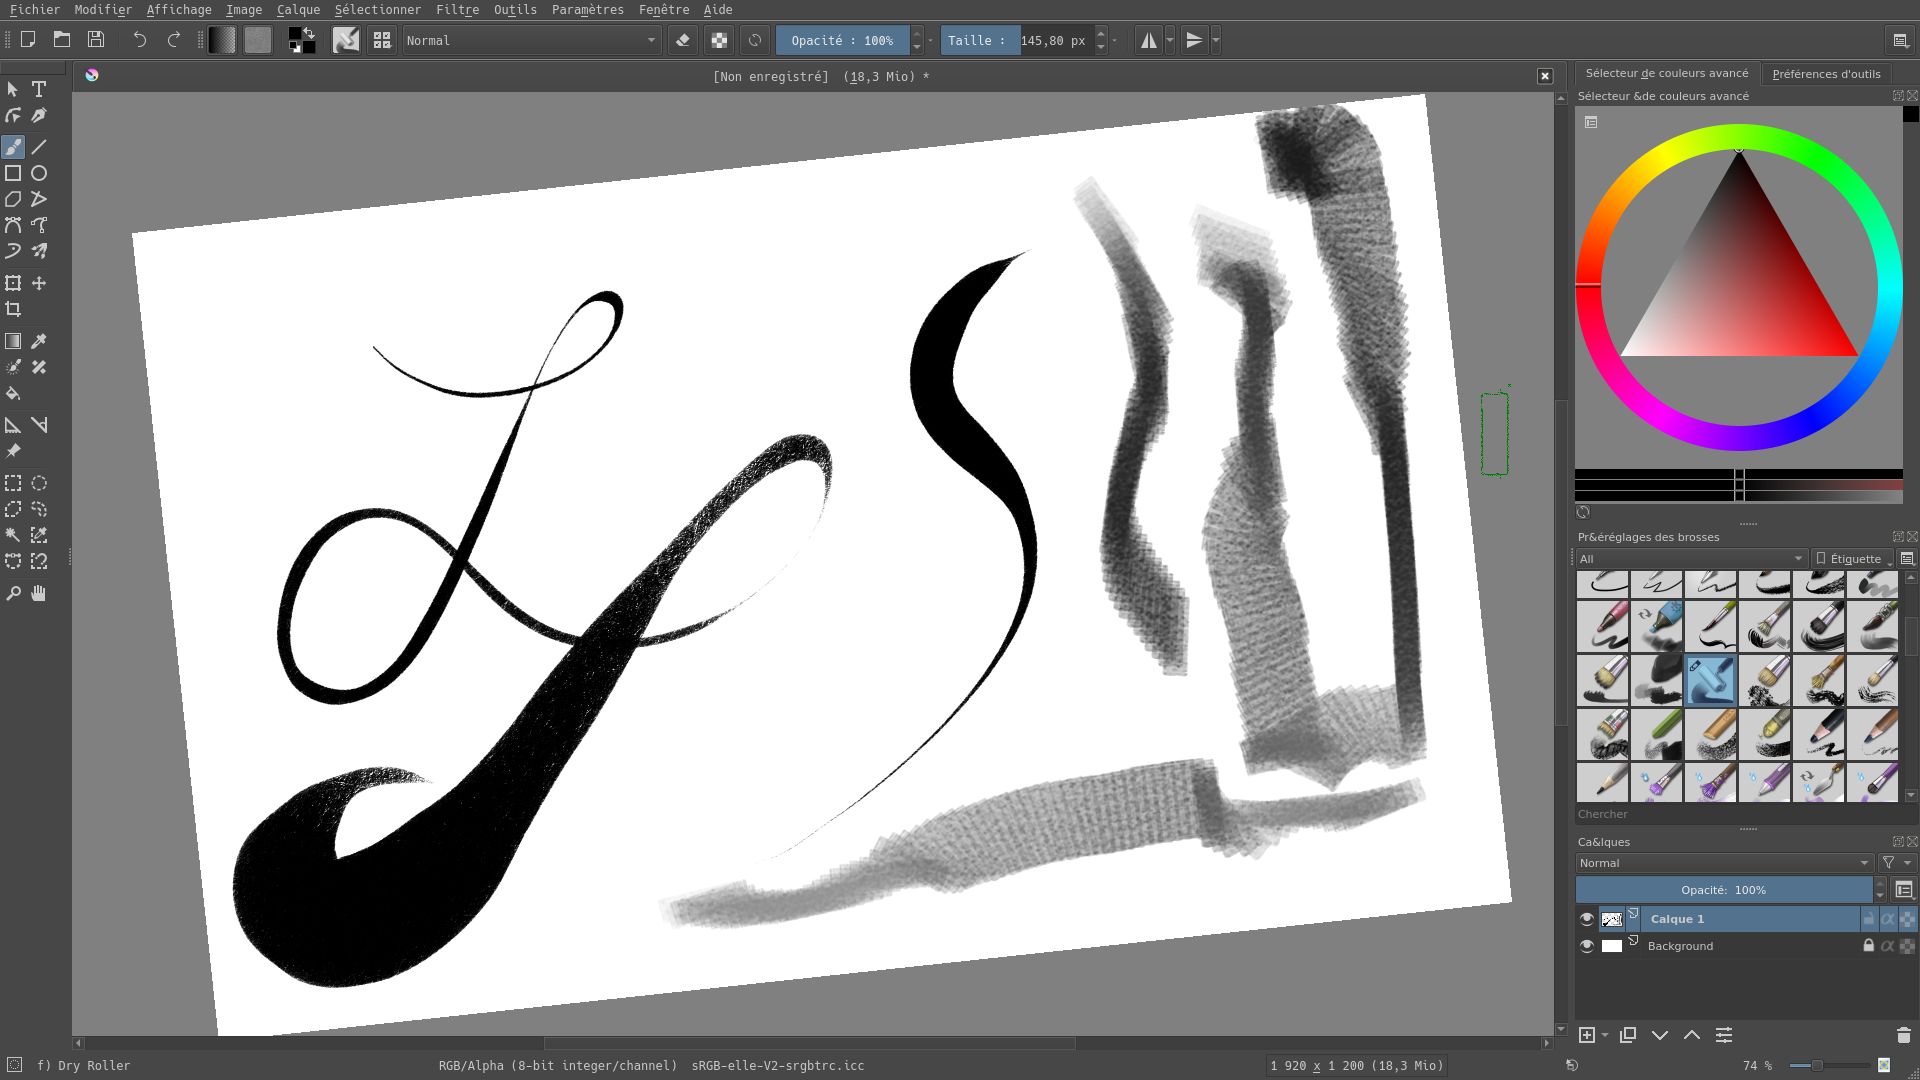
\includegraphics[width=1\paperwidth]{vtb/krita-virtablet.png}}
		\caption{Strokes made in the krita software running on the computer using a galaxy tab s4 running my app and sending the events to the server running on the computer which in turn, injects said events\\
		as you can see, pressure sensitivity and tilt is working.
		the canvas was also rotated using multitouch which was also sent from the tablet and injected by the computer server.
		}
	\end{figure}


\subsection*{\textcolor{purple}{Backend Framework:}}
	I'm working on a backend framework which would allow me to create apps rather quickly, the backend was made in \textbf{Rust} using Actix web and the databases i'm using are scylladb, redis and postgres.
features include authentification module, localisation module based on S2 cells and many more.
the databases used are dependent on compilation flags.
the approach is modular and allow to use and connect individual features in any new project.
I plan on using that framework to build various apps.

i had many more side projects including writing a spiking neural network with dynamic topology (neurons can be created / removed whilst the network is running) library from scratch
but i only put here what i think are the two most relevant.\\
\\
PS: i hope you'll excuse my grammar as it is definitely not the thing i'm the best at.

\end{spacing}
\end{document}
